\documentclass{article}
\usepackage{graphicx} % Required for inserting images
\usepackage{amsmath}

%Required for graphs
\usepackage{pgfplots}
\usetikzlibrary{angles, quotes}
\usetikzlibrary{calc}
\usetikzlibrary{shapes}
\usepackage{wasysym}

\usepackage{tikz}
\usetikzlibrary{shapes.geometric}
\usepackage{amsmath}
\usepackage{amssymb}
\usepackage{xcolor}

\usepackage{multicol}
\usepackage{import}
\usepackage{standalone}

\usepackage{geometry}
 \geometry{ % sets margin and paper size
 a4paper,
 total={170mm,257mm},
 left=27mm,
 right=30mm,
 top=25mm}

\usepackage{subfiles} % Best loaded last in the preamble

\title{VEM summer project}
\author{Rory Yarr}
\date{November 2023}

\begin{document}

\maketitle

\section{Introduction}

\subsection{Poisson problem}
\begin{align*}
    -\Delta{u} & = f \quad  \text{in}\ \ \Omega \\
    u & = 0 \quad  \text{on}\ \delta\Omega
\end{align*}

Where $\Omega \subset \mathbb{R}^n, f \in L^2(\Omega)$ %and $g \in H^{1/2}(\partial\Omega).$

\subsubsection{Variational Form}
The variational problem is to find $ u \in H^1_0(\Omega)$ such that 
\[ a(u,v) = (f,v), \quad \text{for all} \quad v \in H^1_0(\Omega),\]
where 
\[ a(u,v) = \int_{\Omega} \nabla u \cdot \nabla v \,dx, \quad \text{and}\quad 
(f,v) =\int_{\Omega} f v \,dx. \]


\subsection{Virtual Element Space}
Suppose $\mathcal{T}_h$ form a finite sequence of partitions of $\Omega$.
$$V_h:= \{v_h \in H^1_0(\Omega):v_h|_E \in V_h^E\  \forall \, E \in \mathcal{T}_h\}$$  

\subsection{Discrete Bilinear Form}
Define $a^E:H^1(E)\times H^1(E)\rightarrow \mathbb{R}$\\
i.e., $a^h(u,v)=(\nabla u,\nabla v)_{0,E}$
Where $(\cdot,\cdot)_{0,E}$ is the $L^2$ inner product.

\subsection{Ritz projection}
Define the operator $\Pi^E: V_h^E \rightarrow \mathcal{P}_E$,
\begin{enumerate}
    \item $(\nabla(\Pi^Ev_h-v_h),\nabla p)_{0,E} = 0 \hspace{5pt} \forall p \in \mathcal{P_E}$
    \item $\overline{\Pi^Ev_h} = \overline{v_h}$
\end{enumerate}

\begin{align*}
(\nabla\Pi^E_h,\nabla p)_{0,E} &= (\nabla v_h,\nabla p)\\
&= \sum_{e\in \delta E}\int_e v_hn_e\cdot\nabla pds 
&= \sum_{e\in \delta E} v_hn_e\cdot pds 
\end{align*}

$$P_0v_h = \cfrac{1}{|E_k|}\int_{E_k}v_h$$

$\Pi^Ev_h = \sum_{i=1}^{N_k}s^im_i$

\subsection{Basis functions}
Introduce $\{\varphi_i\}^N_{i=1} \in V_h$ as the basis of an element space. This can be computed using Lagrangian polynomial between two points.\\
I.e., $\phi_i = \cfrac{(x_i-x)(y_i-y)}{(x_{i+1}-x_i)(y_{i+1}-y_i)}$



\subsection{Stiffness Matrix K}
For each element $E \in \mathcal{T}_h$
$$K^E = \int_E\nabla\varphi_i\cdot\nabla\varphi_j dE$$

\begin{equation}
    K = \sum_{E \in \mathcal{T}_h}K^E
\end{equation}

\subsection{Load Vector F}

$$F^E = \int_Ef\varphi_i dE$$
\begin{equation}
    F = \sum_{E \in \mathcal{T}_h}F^E
\end{equation}


\section{The Ritz projection and local stiffness matrix}
$G = BD $and$ \tilde{G} = \tilde{B}D$

\section{Calculation of the matrices}

$B_E := \begin{bmatrix}
    P_0\varphi_1 & \hdots & P_0 \varphi_{N^\text{dof}}\\
    (\nabla m_2,\nabla\varphi_1)_{0,E} & \hdots & (\nabla m_2,\nabla\varphi_{N^\text{dof}})_{0,E} \\
    \vdots & \ddots & \vdots \\
    (\nabla m_{n_k},\nabla\varphi_1)_{0,E} & \hdots & (\nabla m_{n_k},\nabla\varphi_{N^\text{dof}})_{0,E}
\end{bmatrix}$
\\

\begin{equation}
    P_0v_h := \cfrac{1}{|E|}\int_E v_h, \text{for} k\geq 2
\end{equation}

\begin{equation}
    m_{\alpha_1,\alpha_2} := \left(\cfrac{x - x_{\mathcal{D}}}{h_{\mathcal{D}}}\right)^{\alpha_1}
    \left(\cfrac{y - y_{\mathcal{D}}}{h_{\mathcal{D}}}\right)^{\alpha_2}
\end{equation}

\begin{equation}
    m_{\alpha} = \left(\cfrac{x-x_\mathcal{D}}{h_\mathcal{D}},\cfrac{y-y_\mathcal{D}}{h_\mathcal{D}}\right)
\end{equation}

\begin{equation}
    D = \begin{pmatrix}
        m_1^E(V_1) & m_x^E(V_1) & m_y^E(V_1) \\
        \vdots & \vdots & \vdots \\
        m_1^E(V_n) & m_x^E(V_n) & m_y^E(V_n) \\
    \end{pmatrix}
\end{equation}


\section{Example}
\documentclass[class=article, crop=false]{standalone}
\usepackage{tikz}
\usepackage{subcaption}
\usetikzlibrary{calc}

\begin{document}
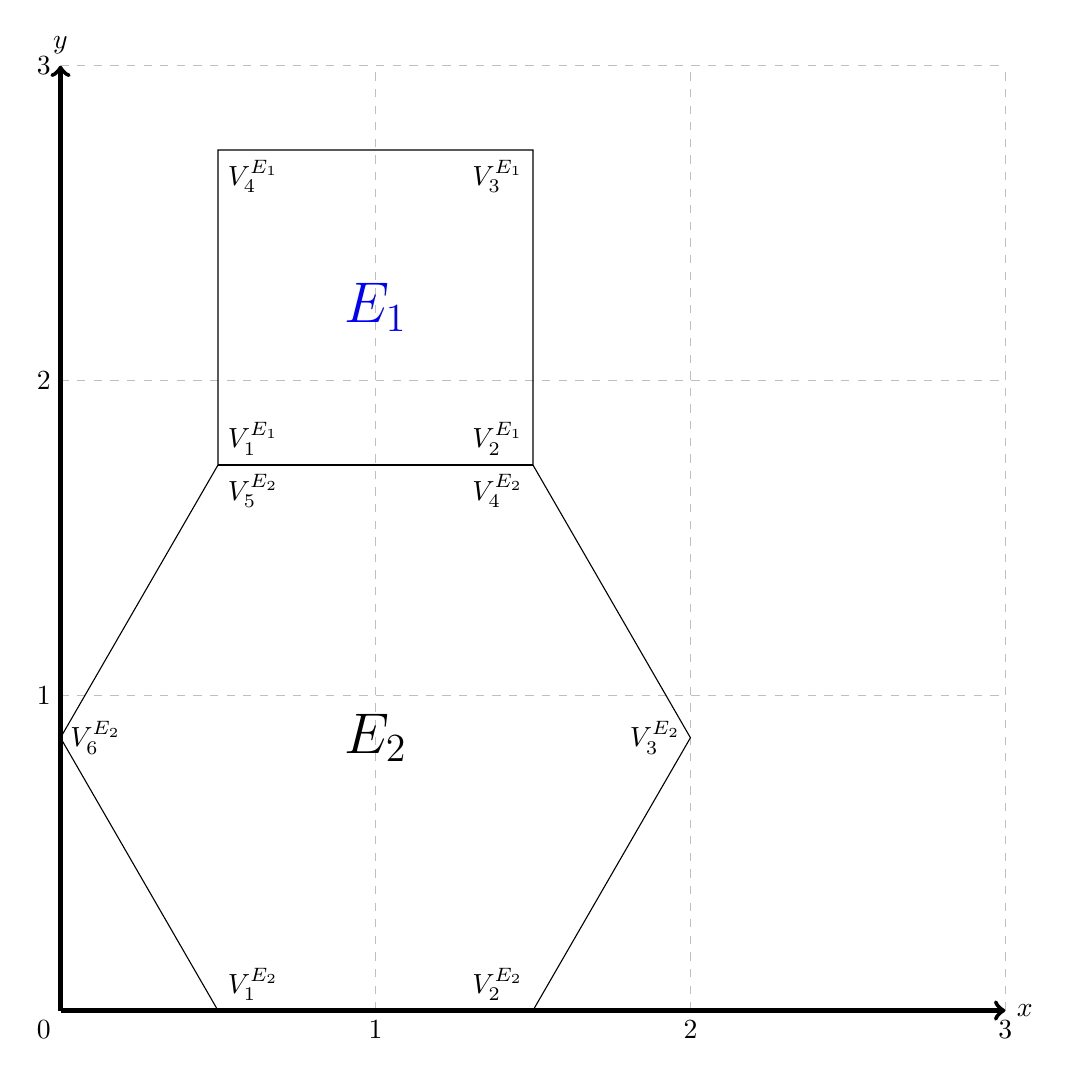
\begin{tikzpicture}[scale=4]
%Define Cooridinates
\coordinate (A) at (0.5,0);
\coordinate (B) at (1.5,0);
\coordinate (C) at (2,0.5*sqrt(3);
\coordinate (D) at (1.5,sqrt(3);
\coordinate (E) at (1.5,1+sqrt(3);
\coordinate (F) at (0.5,1+sqrt(3);
\coordinate (G) at (0.5,sqrt(3);
\coordinate (H) at (0, 0.5*sqrt(3);


%Axis
\draw[help lines, color=gray!50, dashed] (0,0) grid (3,3);
\draw[->,ultra thick] (0,0)--(3,0) node[right]{$x$};
\draw[->,ultra thick] (0,0)--(0,3) node[above]{$y$};

\draw (0,0) node [anchor = north east]{0};

\draw (0,1) node [anchor=east]{1};
\draw (0,2) node [anchor=east]{2};
\draw (0,3) node [anchor=east]{3};

\draw (1,0) node [anchor=north]{1};
\draw (2,0) node [anchor=north]{2};
\draw (3,0) node [anchor=north]{3};


%Lines and vertice labels.
\draw (A) node[anchor=south west]{$V^{E_2}_1$} 
-- (B) node[anchor=south east]{$V^{E_2}_2$} 
-- (C) node[anchor=east]{$V^{E_2}_3$} 
-- (D) node[anchor=north east]{$V^{E_2}_4$} 
-- (E) node[anchor=north east]{$V^{E_1}_3$} 
-- (F) node[anchor=north west]{$V^{E_1}_4$} 
-- (G) node[anchor=north west]{$V^{E_2}_5$} 
-- (H) node[anchor=west]{$V^{E_2}_6$} 
-- (A);
\draw (D) node[anchor=south east]{$V^{E_1}_2$}  
-- (G) node[anchor=south west]{$V^{E_1}_1$} ;

\node[black,rectangle] at (1,0.5*sqrt(3) {\huge $E_2$};
\node[blue,rectangle] at (1,0.5+sqrt(3) {\huge $E_1$};

\end{tikzpicture}
\end{document}

$$E_1 = \begin{cases}
    V_1 = (\frac{1}{2},\sqrt{3}) \\
    V_2 = (\frac{3}{2},\sqrt{3}) \\
    V_3 = (\frac{3}{2},1+\sqrt{3}) \\ 
    V_4 = (\frac{1}{2},1+\sqrt{3}) \\
\end{cases}
\quad
E_2 = \begin{cases}
    V_1 = (\frac{1}{2},0) \\ 
    V_2 = (\frac{3}{2},0) \\ 
    V_3 = (2,\frac{\sqrt{3}}{2}) \\
    V_4 = (\frac{3}{2},\sqrt{3}) \\
    V_5 = (\frac{1}{2}, \sqrt{3}) \\ 
    V_6 = (0, \frac{\sqrt{3}}{2}) \\
\end{cases}$$\\

\subsection{E$_1$}
For $E_1$ the square the coordinates of the centriod are, $x_{E_1} = (1, \frac{1}{2}+\sqrt{3}).$ The diameter is, $ h_{E_1} = \sqrt{2}$ and the area is $|E_1| = 1$.\\

\subsubsection{Momonial basis}
$
m_1^1 = \left(\cfrac{x - 1}{\sqrt{2}}\right)^{0}\left(\cfrac{y -\frac{1}{2} - \sqrt{3}}{\sqrt{2}}\right)^{0} = 1\\
m_x^1 = \left(\cfrac{x - 1}{\sqrt{2}}\right)^{1}\left(\cfrac{y -\frac{1}{2} - \sqrt{3}}{\sqrt{2}}\right)^{0} = \cfrac{x - 1}{\sqrt{2}}\\
m_y^1 = \left(\cfrac{x - 1}{\sqrt{2}}\right)^{0}\left(\cfrac{y -\frac{1}{2} - \sqrt{3}}{\sqrt{2}}\right)^{1} = \cfrac{y - \frac{1}{2} - \sqrt{3}}{\sqrt{2}}$\\


\subsubsection{DOF}

\(
\begin{array}{ll}
m_x^1\bigg|_{x=\frac{1}{2}} = \cfrac{\frac{1}{2} - 1}{\sqrt{2}} = -\cfrac{1}{\sqrt{2}} & \qquad m_y^1\bigg|_{y=\sqrt{3}} = \cfrac{\sqrt{3} - \frac{1}{2} - \sqrt{3}}{\sqrt{2}} = -\cfrac{1}{\sqrt{2}} \\
m_x^1\bigg|_{x=\frac{3}{2}} = \cfrac{\frac{3}{2} - 1}{\sqrt{2}} = \cfrac{1}{\sqrt{2}} & \qquad m_y^1\bigg|_{y=\sqrt{3}+1} = \cfrac{1+\sqrt{3} - \frac{1}{2} - \sqrt{3}}{\sqrt{2}} = \cfrac{1}{\sqrt{2}}
\end{array}
\)

\subsubsection{D$_1$ Matrix}
$D_1 = \cfrac{1}{\sqrt{2}}\begin{pmatrix}
    \sqrt{2} & -1 & -1\\
    \sqrt{2} & 1 & -1\\
    \sqrt{2} & 1 & 1\\
    \sqrt{2} & -1 & 1\\
\end{pmatrix}$

\subsubsection{Gradient of m}
$\nabla m_1^1 = (0,0)$\\
$\nabla m_x^1 = (\frac{1}{\sqrt{2}},0)$ \\
$\nabla m_y^1 = (0,\frac{1}{\sqrt{2}})$ 

\subsubsection{Lagrangian $\mathbf{\phi}$ basis}
$\phi_1 = \cfrac{(x_2-x)(y_4-y)}{(x_2-x_1)(y_4-y_1)}$\\
$\phi_1 = \cfrac{(\frac{3}{2} - x)(1+\sqrt{3} + y)}{(\frac{3}{2}-\frac{1}{2})(1+\sqrt{3} - \sqrt{3})}$\\
Note the denominator is 1 and the same is true for the rest so they can be written in the following form.\\
$\phi_1 = (\frac{3}{2} - x)(1 + \sqrt{3} - y)$\\
$\phi_2 = (x - \frac{1}{2})(1 + \sqrt{3} - y)$\\
$\phi_3 = (x - \frac{1}{2} )(y - \sqrt{3})$\\
$\phi_4 = (\frac{3}{2} - x)(y - \sqrt{3})$

\subsubsection{$P_0\varphi_i$}
$
P_0\varphi_0 = \iint_E(\frac{3}{2} - x)(1+\sqrt{3}-y)dxdy \\
\hspace*{22pt}= \int_{\frac{1}{2}}^{\frac{3}{2}}(\frac{3}{2} - x)dx \int_{\sqrt{3}}^{1+\sqrt{3}}(1+\sqrt{3}-y)dy\\
\hspace*{22pt}= \frac{1}{4}[3x-x^2]_{\frac{1}{2}}^{\frac{3}{2}}[2(1+\sqrt{3})x - x^2]_{\sqrt{3}}^{1+\sqrt{3}}\\
\hspace*{22pt}= \frac{1}{4}(9/2-9/4 - 3/2+1/4)(2(1+\sqrt{3})(1+\sqrt{3})\\
\hspace*{22pt}= \frac{1}{4}(1)(1)$



\subsubsection{Gradient of $\phi$}
$\nabla\phi_1 = \left(-(1 + \sqrt{3} - y),  -(\frac{3}{2}-x)\right)$\\
$\nabla\phi_2 = \left(1 + \sqrt{3} - y,-(x - \frac{1}{2})\right)$\\
$\nabla\phi_3 = \left(y - \sqrt{3},x - \frac{1}{2}\right)$\\
$\nabla\phi_4 = \left(-(y-\sqrt{3}),\frac{3}{2}-x\right)$\\

\subsubsection{$(\nabla m_x,\nabla\phi)$}
$(\nabla m_x^1,\nabla\phi_1)_{E_1} = 
\left(\frac{1}{\sqrt{2}},0\right)\cdot\left(-(1 + \sqrt{3} - y),  -(\frac{3}{2}-x)\right) = 
-\frac{1}{\sqrt{2}}(1 + \sqrt{3} - y)|_{y=\sqrt{3}} = 
-\frac{1}{\sqrt{2}}$\\
$(\nabla m_x^1,\nabla\phi_2)_{E_1} = 
\left(\frac{1}{\sqrt{2}},0\right)\cdot\left(1 + \sqrt{3} - y),  -(x-\frac{1}{2})\right) = 
\frac{1}{\sqrt{2}}(1 + \sqrt{3} - y)|_{y=\sqrt{3}} = 
\frac{1}{\sqrt{2}}$\\
$(\nabla m_x^1,\nabla\phi_3)_{E_1} = 
\left(\frac{1}{\sqrt{2}},0\right)\cdot\left(y-\sqrt{3}, x-\frac{1}{2}\right) = 
\frac{1}{\sqrt{2}}(y-\sqrt{3})|_{y=\sqrt{3}+1} = 
-\frac{1}{\sqrt{2}}$\\
$(\nabla m_x^1,\nabla\phi_3)_{E_1} = 
\left(\frac{1}{\sqrt{2}},0\right)\cdot\left(-(y-\sqrt{3}), \frac{3}{2}-x)\right) = 
-\frac{1}{\sqrt{2}}(y-\sqrt{3})|_{y=\sqrt{3}+1} = 
\frac{1}{\sqrt{2}}$\\


\subsubsection{$\mathbf{(\nabla m_y,\nabla\phi)}$}
$(\nabla m_y^1,\nabla\phi_1)_{E_1} = 
\left(0,\frac{1}{\sqrt{2}}\right)\cdot\left(-(1 + \sqrt{3} - y),  -(\frac{3}{2}-x)\right) = 
-\frac{1}{\sqrt{2}}(\frac{3}{2}-x)|_{x=\frac{1}{2}} = 
-\frac{1}{\sqrt{2}}$\\
$(\nabla m_y^1,\nabla\phi_2)_{E_1} = 
\left(0,\frac{1}{\sqrt{2}}\right)\cdot\left(1 + \sqrt{3} - y),  -(x-\frac{1}{2})\right) = 
-\frac{1}{\sqrt{2}}(x - \frac{1}{2})|_{x=\frac{3}{2}} = 
-\frac{1}{\sqrt{2}}$\\
$(\nabla m_y^1,\nabla\phi_3)_{E_1} = 
\left(0,\frac{1}{\sqrt{2}}\right)\cdot\left(y-\sqrt{3}, x-\frac{1}{2}\right) = 
\frac{1}{\sqrt{2}}(x-\frac{1}{2})|_{x=\frac{3}{2}} = 
\frac{1}{\sqrt{2}}$\\
$(\nabla m_y^1,\nabla\phi_3)_{E_1} = 
\left(0,\frac{1}{\sqrt{2}}\right)\cdot\left(-(y-\sqrt{3}), \frac{3}{2}-x)\right) = 
\frac{1}{\sqrt{2}}(\frac{3}{2}-x)|_{x=\frac{1}{2}} = 
\frac{1}{\sqrt{2}}$\\

\subsubsection{B$_1$ Matrix}
$B_1 = \frac{1}{4}\begin{pmatrix}
    1 & 1 & 1 & 1 \\
    -d & 1 & -1 & 1\\
    -1 & -1 & 1 & 1 
\end{pmatrix}$

\subsubsection{G Matrix}
$G_1 = \begin{pmatrix}
    1
\end{pmatrix}
$

\subsection{E$_2$}
For $E_1$ the square the coordinates of the centriod are, $x_{E_2} = (1,1).$ The diameter is, $ h_{E_1} = 2$ and the area is $|E_1| = \frac{3\sqrt{3}}{2}$.\\
\\
For $m_1^2 = \left(\cfrac{x - 1}{2}\right)^{0}\left(\cfrac{y - 1}{2}\right)^{0} = 1$\\
For $m_x^2 = \left(\cfrac{x - 1}{2}\right)^{1}\left(\cfrac{y - 1}{2}\right)^{0} = \cfrac{(x-1)}{2}$\\
For $m_y^2 = \left(\cfrac{x - 1}{2}\right)^{0}\left(\cfrac{y - 1}{2}\right)^{1} = \cfrac{y-1}{2}$\\

\subsubsection{Monimals}
$\begin{array}{ll}
m_x^2|_{x=0}\hspace{1.5pt} = \cfrac{0-1}{2} = -\frac{1}{2} &\qquad m_y^2|_{y=0} \hspace{7pt}= \cfrac{0-1}{2} = -\frac{1}{2} \\
m_x^2|_{x=\frac{1}{2}} = \cfrac{\frac{1}{2}-1}{2} = -\frac{1}{4} &\qquad m_y^2|_{y=\frac{\sqrt{3}}{2}} = \cfrac{\frac{\sqrt{3}}{2}-1}{2} = \frac{\sqrt{3}-2}{4} \\
m_x^2|_{x=\frac{3}{2}} = \cfrac{\frac{3}{2}-1}{2} = \frac{1}{4} &\qquad m_y^2|_{y=\sqrt{3}}\, = \cfrac{\sqrt{3}-1}{2} = \frac{\sqrt{3}-1}{2} \\
m_x^2|_{x=2}\hspace{1.5pt} = \cfrac{2-1}{2} = \frac{1}{2} &
\end{array}$

$D_2 = \cfrac{1}{4}\begin{pmatrix}
    4 & -1 & - 2\\
    4 & 1 & - 2\\
    4 & 2 & \sqrt{3} - 2\\
    4 & 1 & 2\sqrt{3} - 2\\
    4 & -1 & 2\sqrt{2} - 2\\
    4 & -2 & \sqrt{3} - 2\\
\end{pmatrix}$

\subsection{B matrix}
$\nabla m_1^2 = (0,0)$\\
$\nabla m_x^2 = (\frac{1}{2},0)$ \\
$\nabla m_y^2 = (0,\frac{1}{2})$ \\

Hence, \\
$P_0m_1 = \int_E\frac{1}{E}$

\subsection{Mesh example.}
The mesh is defined using 3 sets, Vertices, Elements and Boundary. The first is an array of coordinates for each node. The Vertices element set contains a vector for each element. With the index for each node in the element labeled anti-clockwise. The boundary is a vector containing the indices in an anticlockwise order.




%\subfile{Matlab/FunctionsUsed}

\section{Appendix}
%\subfile{Matlab/VEM}

\begin{verbatim}

function u = vem(mesh_filepath, rhs, boundary_condition)
% VEM computes the virtual element solution of a Poisson problem on a polygonal mesh
%
% SYNOPSIS: u = vem(mesh_filepath, rhs, boundary_condition)
%
% INPUT: mesh_filepath:		A string specifying the path to a mesh file
%	 rhs:			A handle to a function specifying the PDE 
% 				forcing function
%	 boundary_condition:	A handle to a function specifying the 
% 				boundary condition of the PDE
% 
% OUTPUT: u: A vector of the the degrees of freedom of the virtual element 
%		solution to the PDE
% 
% EXAMPLE:
%  u = vem('meshes/L-domain.mat', @L_domain_rhs, @L_domain_boundary_condition)

% AUTHOR: Oliver Sutton, 2016

mesh = load(mesh_filepath); % Load the mesh from a .mat file
n_dofs = size(mesh.vertices, 1); n_polys = 3; % Method has 1 degree of freedom per vertex
K = sparse(n_dofs, n_dofs); % Stiffness matrix
F = zeros(n_dofs, 1); % Forcing vector
u = zeros(n_dofs, 1); % Degrees of freedom of the virtual element solution
linear_polynomials = {[0,0], [1,0], [0,1]}; % Impose an ordering on the linear polynomials
mod_wrap = @(x, a) mod(x-1, a) + 1; % A utility function for wrapping around a vector
for el_id = 1:length(mesh.elements)
	vert_ids = mesh.elements{el_id}; % Global IDs of the vertices of this element
	verts = mesh.vertices(vert_ids, :); % Coordinates of the vertices of this element
	n_sides = length(vert_ids); % Start computing the geometric information
	area_components = verts(:,1) .* verts([2:end,1],2) - verts([2:end,1],1) .* verts(:,2);
	area = 0.5 * abs(sum(area_components));
	centroid = sum((verts + verts([2:end,1],:)) .* repmat(area_components,1,2)) / (6*area);
	diameter = 0; % Compute the diameter by looking at every pair of vertices
	for i = 1:(n_sides-1)
		for j = (i+1):n_sides
			diameter = max(diameter, norm(verts(i, :) - verts(j, :)));
		end
	end
	D = zeros(n_sides, n_polys); D(:, 1) = 1;
	B = zeros(n_polys, n_sides); B(1, :) = 1/n_sides;
	for vertex_id = 1:n_sides
		vert = verts(vertex_id, :); % This vertex and its neighbours
		prev = verts(mod_wrap(vertex_id - 1, n_sides), :);
		next = verts(mod_wrap(vertex_id + 1, n_sides), :);
		vertex_normal = [next(2) - prev(2), prev(1) - next(1)]; % Average of edge normals
		for poly_id = 2:n_polys % Only need to loop over non-constant polynomials
			poly_degree = linear_polynomials{poly_id};
			monomial_grad = poly_degree / diameter; % Gradient of a linear is constant
			D(vertex_id, poly_id) = dot(vert - centroid, poly_degree) / diameter;
			B(poly_id, vertex_id) = 0.5 * dot(monomial_grad, vertex_normal);
		end
	end
	projector = (B*D) \ B; % Compute the local Ritz projector to polynomials
	stabilising_term = (eye(n_sides) - D * projector)' * (eye(n_sides) - D * projector);
	G = B*D; G(1, :) = 0;
	local_stiffness = projector' * G * projector + stabilising_term;
	K(vert_ids,vert_ids) = K(vert_ids,vert_ids) + local_stiffness; % Copy local to global
	F(vert_ids) = F(vert_ids) + rhs(centroid) * area / n_sides;
end
boundary_vals = boundary_condition(mesh.vertices(mesh.boundary, :));
internal_dofs = ~ismember(1:n_dofs, mesh.boundary); % Vertices which aren't on the boundary
F = F - K(:, mesh.boundary) * boundary_vals; % Apply the boundary condition
u(internal_dofs) = K(internal_dofs, internal_dofs) \ F(internal_dofs); % Solve
u(mesh.boundary) = boundary_vals; % Set the boundary values
plot_solution(mesh, u)
end
\end{verbatim}

\end{document}
